\documentclass[border=3pt,tikz]{standalone}
\usepackage{amsmath}
\usetikzlibrary{arrows}
\usetikzlibrary{positioning}
\usetikzlibrary{calc}
\usetikzlibrary{arrows}
\begin{document}
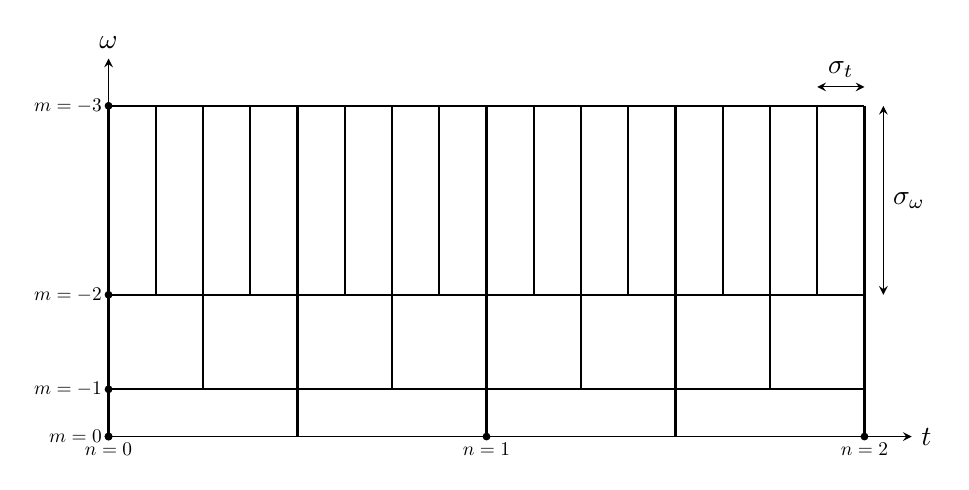
\begin{tikzpicture}[samples = 200, scale=1.2]

    \draw[-{stealth}] (0, 0) -- (8.5,0) node[right] {$t$};
    \draw[-{stealth}] (0,0) -- (0,4) node[above] {$\omega$};
    
    \draw [thick] (0, 0.5) -- (8, 0.5);
    \draw [thick] (0, 1.5) -- (8, 1.5);
    \draw [thick] (0, 3.5) -- (8, 3.5);
    
    
    \filldraw[black] (0, 0) circle (1pt) node [below, scale=0.7] {$n=0$};
    \filldraw[black] (4, 0) circle (1pt) node [below, scale=0.7] {$n=1$};
    \filldraw[black] (8, 0) circle (1pt) node [below, scale=0.7] {$n=2$};
    \filldraw[black] (0, 0) circle (1pt) node [left, scale=0.7] {$m=0$};
    \filldraw[black] (0, 0.5) circle (1pt) node [left, scale=0.7] {$m=-1$};
    \filldraw[black] (0, 1.5) circle (1pt) node [left, scale=0.7] {$m=-2$};
    \filldraw[black] (0, 3.5) circle (1pt) node [left, scale=0.7] {$m=-3$};
    
    \foreach \x in {0,...,4}
    {
    \draw [thick] (2*\x, 0) -- (2*\x, 3.5);
    
    }
    
    
    \foreach \x in {0,...,8}
    {
    \draw [thick] (\x, 0.5) -- (\x, 3.5);
    }
    
    \foreach \x in {0,...,15}
    {
    \draw [thick] (\x/2, 1.5) -- (\x/2, 3.5);
    }
    
    \draw[{stealth}-{stealth}] (7.5, 3.7) -- (8.0,3.7);
    \node[above] at (7.75, 3.7) {$\sigma_t$};
    
    \draw[{stealth}-{stealth}] (8.2, 1.5) -- (8.2,3.5);
    \node[right] at (8.2, 2.5) {$\sigma_\omega$};
    
    \end{tikzpicture}
\end{document}